\documentclass[titlepage]{report}

\usepackage[margin=1in]{geometry}
\usepackage{fancyhdr}
\usepackage{csquotes}
\usepackage{marginnote}
\usepackage{scrextend}
\usepackage[bottom]{footmisc}
\usepackage{enumitem}
\usepackage{xr}
\usepackage{amsmath,amssymb,amsthm}
\usepackage{mathtools,physics}
\usepackage{tikz,graphicx,subcaption}
\usepackage[hidelinks]{hyperref}

\fancypagestyle{plain}{
    \fancyhead{}
    \renewcommand{\headrulewidth}{0pt}
}
\fancypagestyle{main}{
    \fancyhf{}
    \fancyhead[L]{\leftmark}
    \fancyhead[R]{MATH 16110}
    \fancyfoot[R]{Labalme \thepage}
}

\MakeOuterQuote{"}

\reversemarginpar

\deffootnotemark{\textsuperscript{\textup{[}\thefootnotemark\textup{]}}}
\deffootnote[2.1em]{0em}{0em}{\textsuperscript{\thefootnote}}

\setitemize[3]{label={\scriptsize$\blacksquare$}}

\DeclareMathOperator{\ext}{ext}

\newtheorem{theorem}{Theorem}[chapter]
\newtheorem{proposition}[theorem]{Proposition}
\newtheorem{lemma}[theorem]{Lemma}
\newtheorem{corollary}[theorem]{Corollary}
\newtheorem{axiom}{Axiom}
\newtheorem*{axioms}{Axioms}
\newtheorem*{theorem*}{Theorem}
\newtheorem*{lemma*}{Lemma}
\newtheorem{lemmaM}{Lemma}
\newtheorem{corollaryM}{Corollary}
\theoremstyle{definition}
\newtheorem{definition}[theorem]{Definition}
\newtheorem{exercise}[theorem]{Exercise}
\newtheorem{remark}[theorem]{Remark}
\newtheorem*{definition*}{Definition}
\newtheorem{exerciseM}{Exercise}

\usetikzlibrary{positioning,shapes,decorations.pathreplacing,calc}

\renewcommand{\chaptername}{Script}

\newcommand{\N}{\mathbb{N}}
\newcommand{\Z}{\mathbb{Z}}
\newcommand{\mA}{\mathcal{A}}
\newcommand{\Q}{\mathbb{Q}}
\newcommand{\eqclass}[2]{\left[ \frac{#1}{#2} \right]}
\newcommand{\plusQ}{+_\Q}
\newcommand{\cdotQ}{\cdot_\Q}
\newcommand{\lQ}{<_\Q}

\usepackage{subfiles}

\title{MATH 16110 (Honors Calculus I IBL) Notes}
\author{Steven Labalme}

\begin{document}




\maketitle



\pagenumbering{roman}
\tableofcontents
\listoffigures
\newpage



\pagenumbering{arabic}
\pagestyle{main}
\subfile{NotesOnProofs/notesonproofs.tex}



\setcounter{secnumdepth}{3}
\subfile{Script0/script0.tex}


\section{Discussion}
\begin{itemize}
    \item \marginnote{10/8:}How much of the proof of Additional Exercise \ref{axr:0.7} proof could be left out as unnecessary verbage?
\end{itemize}



\subfile{Script1/script1.tex}


\section{Discussion}
\begin{itemize}
    \item \marginnote{10/1:}Always make sure you use all given assumptions.
    \item We are allowed to assume that $x\in\{A:Q\}$ tells us that $x\in A$ and $Q$ is true? --- yes.
    \item We can let $x$ be an arbitrary element of a set and deduce stuff like in Tao.
    \item When we're writing proofs (consider Theorem \ref{trm:1.12}), do we do not have to show the definition of $A\cap B$? --- we can just say "by Definition \ref{dfn:1.6}, $y\notin A\cap B$ implies that $y\notin a$ or $y\notin b$."
    \begin{figure}[h!]
        \centering
        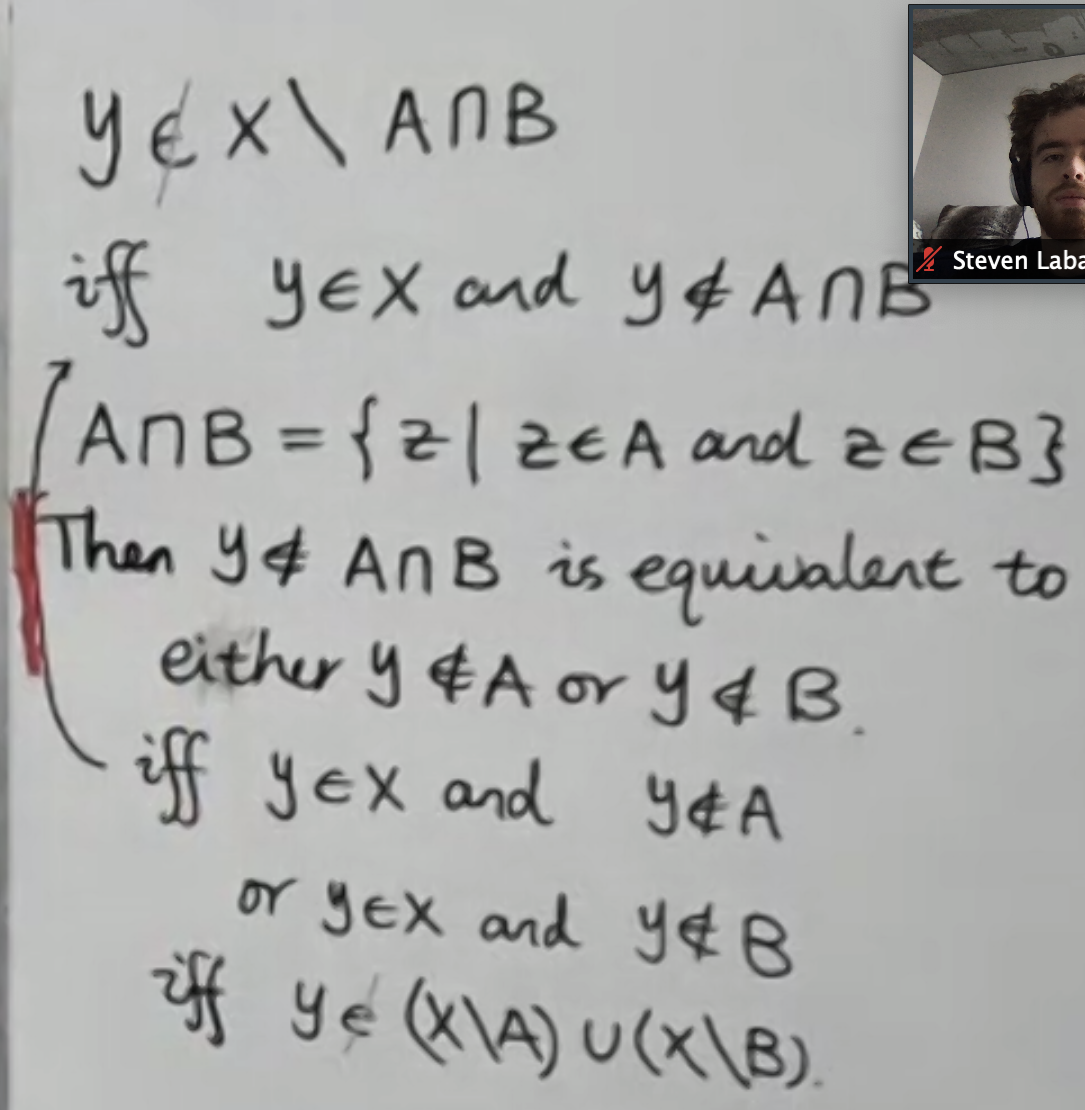
\includegraphics[width=0.3\linewidth]{ExtFiles/SampleTrm1-12Proof.png}
        \caption{Sample exam-ready proof of Theorem \ref{trm:1.12}.}
        \label{fig:sampleTrm1-12Proof}
    \end{figure}
    \item What he wrote for the beginning of the proof of Theorem \ref{trm:1.12} (see Figure \ref{fig:sampleTrm1-12Proof}) is acceptable on an exam; in our exams, it will be the same as when presenting to class (we do not need complete sentences).
    \item Can we say "A similar argument works in reverse?"
    \item \marginnote{10/6:}Vacuous truths were introduced.
    \item If you had to prove your answers to Additional Exercise \ref{axr:1.1}, you would write out the elements of the first set, and rewrite the elements with each additional constraint.
    \begin{itemize}
        \item For example, $(\{n\in\Z\mid n\text{ is divisible by }2\}\cap\N)\cup\{-5\}=(\{\cdots,-4,-2,0,2,4,\cdots\}\cap\{1,2,3,\cdots\})\cup\{-5\}=\{2,4,6,\cdots\}\cup\{-5\}$.
    \end{itemize}
    \item In this class, $0\notin\N$, but $0\in\N_0$.
    \item For Exercise \ref{exr:1.21}, we can refer to Theorem 7 in "Notes on proofs" to demonstrate that $\sqrt{2}\notin\N$.
    \item When presenting, write on the board more like I would in a journal.
    \item Ask about my contradiction proofs for 1.21-1.23!
    \item \marginnote{10/8:}! means "unique."
    \item $\because$ means "since."
    \item \marginnote{10/13:}What are your office hours? Mondays 4-6 PM.
    \item Do I need to submit the LaTeX assignment to you? Email it to him!
    \item Edit this document to reflect switch to section 22!
    \item Script \ref{sct:2} sign up sheet is on Canvas (sign up within 24 hours)!
    \item \marginnote{10/15:}Informal explanation of $10^a+10^b=10^c+10^d$ is ok.
\end{itemize}



\subfile{Script2/script2.tex}


\section{Discussion}
\begin{itemize}
    \item \marginnote{10/15:}Divisibility (see Exercise \ref{exr:2.2d}) is defined in terms of multiplication in Script \ref{sct:0}. Thus, I should use $y-x=5a$ for some $a\in X$ instead of $\frac{y-x}{5}\in X$.
    \item At the end of the proof of Exercise \ref{exr:2.2e}, do casework on $c$ ($c=0$ and $c\neq 0$) to stymie accusations of dividing by 0.
    \item Exercise \ref{exr:2.6}:
    \begin{itemize}
        \item Note that we cannot always pick an arbitrary element of a set (e.g., if a set is empty). However, by definition, $\eqclass{a}{b}$ is nonempty, so we \emph{can} pick an arbitrary element in it.
        \begin{itemize}
            \item Additionally, note that we are probably fine not getting into this technicality because performing any operation on a hypothetical $x\in\emptyset$ invokes vacuous (i.e., weird but still sound) logic.
        \end{itemize}
        \item Let $(x_1,x_2)$ be an arbitrary element of the left set. It is therefore related to $(a,b)$. By set equality, it is an element of the right set. Thus, $(x_1,x_2)\sim(a',b')$. Use symmetry/transitivity to show $(a,b)\sim(a',b')$.
    \end{itemize}
    \item Rewrite Theorem \ref{trm:2.8} as a direct proof.
    \item Journal format: Turning in what I have in this document is fine.
    \item \marginnote{10/20:}Edit Exercise \ref{exr:2.2d} to use Additional Exercise \ref{axr:0.8-i}!
    \item Do we have to prove injectivity for $h$ in Theorem \ref{trm:2.11}? (Injectivity implies bijectivity by Exercise \ref{exr:1.38}.)
    \begin{itemize}
        \item Yes, we still have to prove injectivity here.
    \end{itemize}
    \item Technically, you have to prove that $\N$ is countable, but Cartee won't be looking for it --- you won't have to prove it for credit.
    \item You can also use a lemma that a surjection $f:A\to B$ where $A$ is countable and $B$ is infinite implies that $B$ is countable.
    \item $\gcd(a,b)$ is defined as the largest natural number by which $a$ and $b$ are both divisible.
    \item We want to pick the pair in the equivalence class that has the lowest possible, positive denominator. Think about it in terms of the well-ordering principle. You get a huge set of pairs, look at the subset with positive denominators, then look at just the denominators. You would have to explain why one denominator corresponds to one ordered pair.
    \item Use $f(\eqclass{a}{b})=(a',b')$ to denote that $a\neq a'$ and $b\neq b'$ in every case although the numbers are related.
    \item Two things in the same equivalence class go to the same place, whereas two things in different equivalent classes go to different places.
    \item We're restricting the range with the well-ordering principle, not the domain.
\end{itemize}



\subfile{Script3/script3.tex}


\section{Discussion}
\begin{itemize}
    \item \marginnote{10/20:}Show that $|\{x\}|=1$? Perhaps in a lemma by defining a singleton set. Also make sure that it's clear that $A\cap\{x\}=\emptyset$ to use Theorem \ref{trm:1.34b}.
    \begin{itemize}
        \item Using $B=A\setminus\{x\}$ might help in identifying that $x$ exists, and would help in $B\cap\{x\}=\emptyset$. Thus, $|\{x\}|+|B|=|A|$, it follows by subtraction that $|B|=n$. Potentially as a lemma so I can use it in Theorem \ref{trm:3.5}, too?
    \end{itemize}
    \item Consider case in Theorem \ref{trm:3.5} that $A$ is empty.
    \item What is a limit point?
    \begin{itemize}
        \item A point $p$ would be a limit point of a set $A$ if there's a point $p$ to which the elements of $A$ converge. So on an open interval, the limit points would be the two "end points" and every point therein.
        \item No limit points on the integers. Yes on the rationals and reals.
    \end{itemize}
    \item \marginnote{10/22:}For Exercises \ref{exr:3.9a} and \ref{exr:3.9c}, it is necessary to show that at least one of the three trichotomy statements holds.
    \item \marginnote{10/27:}Do we have to show the explicit proof of both cases in the second part of Lemma \ref{lem:3.16}, or can we just say, "the proof is symmetric?"
\end{itemize}




\end{document}